\documentclass[a4paper, titlepage]{article}

\usepackage{graphicx}
\usepackage{lipsum} % handling margins and formatting of the entire document
\usepackage[margin=1.5in, includefoot]{geometry}
\usepackage[urlcolor=blue]{hyperref}

% Header and Footer Stuff
\usepackage{fancyhdr}
\pagestyle{fancy}
\fancyhead{}
\fancyfoot{}                        % Delete the current footer
\fancyfoot[R]{\thepage}             % Aligns page number to the right on the footer
\renewcommand{\headrulewidth}{0pt}  % 0pt hides the header line, xpt will create a header line x pt size
\renewcommand{\footrulewidth}{0pt}  % 0pt hides the footer line, xpt will create a footer line x pt size
\graphicspath{{images/}}

% custom code snippet formatting
\usepackage{listings}

\begin{document}
\begin{titlepage}
    \begin{center}
        \includegraphics[width=0.5\linewidth]{Towers-watson}
        \line(1,0){300} \\
        [0.25in]
        \huge{\bfseries Security Training} \\
        [2mm]
        \line(1,0){300} \\
        [10cm]
    \end{center}
    \begin{flushright}
        \textsc{\large Jacob Meline } \\
        \today
    \end{flushright}
\end{titlepage}

% Table of Contents %
\tableofcontents
\thispagestyle{empty}
\cleardoublepage
\setcounter{page}{1}

% Introduction %
\section{Introduction}\label{sec:intro}
Some useful terms to know:
\begin{description}
    \item[OWASP] The Open Web Application Security Project. Is an online community dedicated to web application security. Participants include corporations, educational organizations, and individuals.

    \item[PHI] Protected Health Information
    \begin{enumerate}
        \item The individual's past, present, or future physical or mental health or condition.
        \item The Provision of health care to the individual, or
        \item the past, present, or future payment for the provision of health care to the individual,
        \item the individual's identity or for which there is a reasonable basis to believe it can be used to identify the individual
    \end{enumerate}
    \item[PII] Personal Identifiable Information
    \begin{enumerate}
        \item Social Security Number
        \item Driver's license or California Identification Card Number
        \item Account number, credit or debit card number, in combination with any required security code, access code, or password that would permit access to an individual's financial account
    \end{enumerate}

\end{description}

\newpage

% ---------------------------SQL Injection------------------------------------%
\section{SQL Injection A1}

\subsection{What is SQL Injection}
A simple example could look like this: `http://mysite.com/color?colorid=4`
It doesn't matter what site it is, this site has a path called "color" with a query string called "colorid" with a value of 4. The query probably looks like something like this. "select * from color where colorid=4"

"4" is data. It is untrusted. \ it comes in via the url. Changing "4" to "5" will give you a different color

Internal errors can give hackers an idea of what is allowed in your database or not.

\subsection{Why SQL Injection Matters}

Discoverability EASY, Prevalence COMMON, Exploitability EASY, Impact SEVERE

Further readings:

\begin{itemize}
    \item \href{https://www.acunetix.com/websitesecurity/sql-injection/}{acunetix's article}
\end{itemize}

\subsection{Why is SQL Injection a problem?}

Example of attack
\begin{itemize}
    \item \href{http://www.w3schools.com/sql/sql_injection.asp}{A simple example of SQLi}
    \item \href{https://www.hackthissite.org/missions/realistic/4/}{A more realistic example}
    \item \href{https://www.hackthissite.org/missions/realistic/2/}{Another realistic example}
\end{itemize}

In the first hackthissite example, we first have to look everywhere in the site.
\begin{description}
    \item[Investigate the Site]
        \begin{description}
            \item[Source Code] You have to dig through the code. A lot of modern sites will have tests to stop sqlinjection. But you still need to watch out for vulnerabilities. By looking through the source code, you can sometimes find some pretty serious issues. The input is clearly visible. The first step is to attempt to get out of the string. Try registering an email address contatining apostrophes, both single and double. By trying different combinations, we get a different type of message. "Error inserting into table "email"! Email not Valid. Please contact an administrator of Fischer's
            \item[Check the other pages] Looking at the other products, both are using products.php with the category ID as an argument. You can change the argument to be ?category=2 or category=1 to get a combination of both pages on the same page.

        \end{description}
\end{description}


Lets say that a form is asking for user credentials and enter "Tom," well, that is fine and all. If you enter Tom" you're going to have some vulunerability concerns. You can do Tom"; DROP ALL DATABASES; to do some serious damage. To mitigate this attack, you can simply put a slash before any quotation mark. This forces SQL to read it as a quotation mark and not a continuation of a command.

\subsection{How to mitigate SQLi attacks?}
Links to useful sites
\begin{itemize}
    \item \href{https://www.owasp.org/index.php/SQL_Injection_Prevention_Cheat_Sheet}{SQLi Prevention Cheat Sheet}
\end{itemize}
\newpage

% ---------------------------SQL Injection End------------------------------------%

% ---------------------------Cross Site Request Forgery ------------------------------------%
\section{Cross Site Request Forgery}
\subsection{What is Cross-Site Request Forgery}
A CSRF attack forces a logged-on victim's browser to send a forged HTTP request, including the victim's session cookie and any other automatically included authentication information, to a vulnerable web application. This allows the attacker to force the victim's broswer to generate requests the vulnerable application thinks are legitimate requests from the victim.

\newpage


% ---------------------------Cross Site Request Forgery End------------------------------------%
% ---------------------------Cross Site Scripting / XSS------------------------------------%
\section{Cross Site Scripting}

Cross-Site Scripting is a vulnerability that doesn't sanitize user input properly. It allows an attacker to inject HTML or client side script such as Javascript into a website. It is commonly used to steal cookies. Cookies are used for authenticating, tracking, and maintaining specific information about users. There are three different types of Cross Site Scripting:
\begin{description}
    \item [Persistent] \hfill \\
        the malicious input originates from the website's database.
    \item [Non-Persistent]\hfill \\
        the malicious input originates from the victim's request.
    \item [DOM-Based]\hfill \\
        the vulnerability is in the client-side code rather than the server-side code.
\end{description}

\subsection{How to mitigate Cross-Site Scripting}
\begin{itemize}
    \item The most important way to prevent XSS attacks is to perform secure input handling.
        \begin{itemize}
            \item Most of the time, encoding should be performed whenever user input happens
            \item In some cases, encoding has to be replaced by or complemented with validation
            \item Secure input handling has to take into account which context of a page the user input is inserted into
            \item To prevent all types of XSS attacks, secure input handling has to be performed in both client-side and server-side code
        \end{itemize}
    \item Content Security Policy provides an additional layer of defense for when secure input handling fails
\end{itemize}
\newpage

% ---------------------------Click jacking-----------------------------------%
\section{Clickjacking}
\subsection{What is Clickjacking?}
OWASP gives a good example of what click jacking is:

Imagine an attacker who builds a web site that has a button on it that says "click here for a free iPod". However, on top of that web page, the attacker has loaded an iframe with your mail account, and lined up exactly the "delete all messages" button directly on top of the "free iPod" button. The victim tries to click on the "free iPod" button but instead actually clicked on the invisible "delete all messages" button. In essence, the attacker has "hijacked" the user's click, hence the name "Clickjacking".  \newline
\begin{center}
\textbf{Basic ingredients to prepare for a clickjacking attack are}: \newline
\line(1,0){300} \\

\begin{description}
    \item[Iframe] This is a frame in the HTML that frames a webpage in it
    \item[Z-Index] Decides the iframe index in the stack
    \item[Opacity] Makes the iframe transparent
    \item[Position:Absolute] Lines up the iframe with the dummy page
\end{description}
\end{center}
\subsection{How to mitigate against it?}

\begin{itemize}
    \item Sending the proper X-Frame-Options HTTP response headers that instruct the browser to not allow framing from other domains
    \item Employing defensive code in the UI to ensure that the current frame is the most top level window
    \begin{itemize}
        \item Frame-breaker
        By inserting this script into the header of your site, it is an easy way to break the iframe.
        \begin{lstlisting}

        <script>
        if (top != self){ top.location = self.location; }
        </script>

        \end{lstlisting}
    \end{itemize}
\end{itemize}
\newpage

% ---------------------------Click jacking end-----------------------------------%
\section{Authentication}
All approaches for human authentication rely on at least one of the following
\newline
\newline
\textbf{Multi Authenication}
\begin{description}
    \item[Something you know (eg. a password)] This is the most common kind of authentication used for humans. We use passwords every day to access our systems. Unfortunately, something that you know can become something you just forgot. And if you write it down, then other people might find it.
    \item [Something you have (eg. a smart card)] This form of human authentication removes the problem of forgetting something you know, but some object now must be with you any time you want to be authenticated. And such an object might be stolen and then becomes something the attacker has.
    \item [Something you are (eg. a fingerprint)] Base authentication on something intrinsic to the principal being authenticated. It's much harder to lose a fingerprint than a wallet. Unfortunately, biometric sensors are fairly expensive and (at present) not very accurate.
\end{description}

\subsection{Account Lockout}

In an account lockout attack, an attacker attempts to lock out user accounts by purposely failing the authentication process as many times as needed to trigger the account lockout functionality. This in turn prevents even the valid user from obtaining access to their account. For example, if an account lockout policy states that users are locked out of their accounts after three failed login attempts, an attacker can lock out accounts by deliberately sending an invalid password three times. On a large scale, this attack can be used as one method in launching a denial of service attack on many accounts. The impact of such an attack is compounded when there is a significant amount of work required to unlock the accounts to allow users to attempt to authenticate again.

\subsubsection{Ebay Account Lockout Attack}
At one time, eBay displayed the user-id of the highest bidder for a given auction. In the final minutes of the auction, an attacker who was wanting to outbid the current highest bidder could attempt to authenticate three times using the targeted account. After three deliberately incorrect authentication attempts, eBay password throttling would lock out the highest bidder's account for a certain amount of time. An attacker could then make their own bid and the legitimate user would not have a chance to place a counter-bid because they would be locked out of their account.

\subsubsection{Mitigation Strategies}
Brute force attacks are surprisingly difficult to completely mitigate. Careful design and implementation will assist in helping to minimize these attacks.
\begin{itemize}
    \item Since passwords are not always the best option. Having a public-private key setup (Something you have) can help in some circumstances
    \item Time-increasing failed login. For example, after 3 unsuccessful logins, you could block the login for this account for 30 seconds. After the 30 seconds, if the 4th login is still unsuccessful, you stop it for 1 minute, then 5m, and you increase more and more
\end{itemize}

\subsection{Passwords and Hashes}
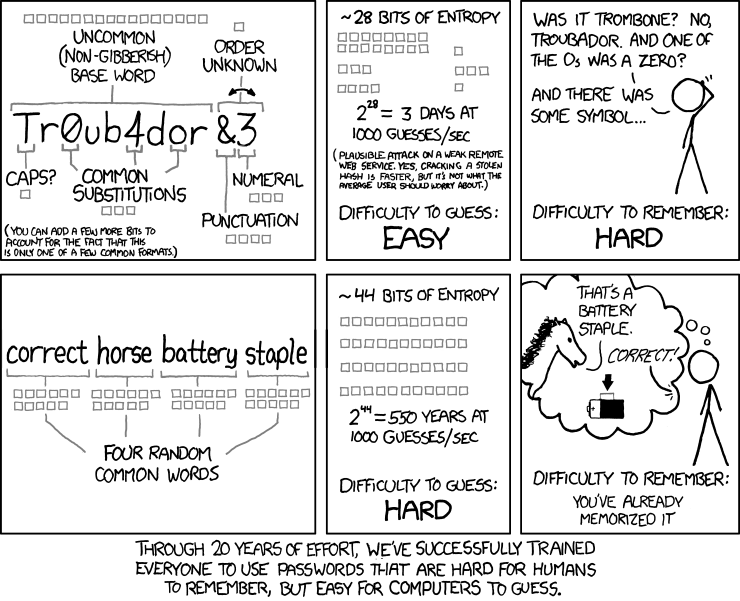
\includegraphics[width=\textwidth]{password_strength}
Sources:
\begin{itemize}
    \item \href{http://www.unixmen.com/john-the-ripper-the-fast-multi-platform-password-cracking-tool/}{John the ripper}
    \item \href{http://blog.codinghorror.com/your-password-is-too-damn-short/}{Your password is too short}
    \item \href{http://null-byte.wonderhowto.com/how-to/hack-like-pro-crack-passwords-part-1-principles-technologies-0156136/}{cracking passwords like a pro}

\end{itemize}
\subsection{Password History}

It is typical in a company to require its employees to have a new password every 6 - 12 months. On top of that, there can be time restrictions on the previous passwords so that even if old passwords were compromised, attackers wouldn't be able to brute force their way through a secure network.

\subsection{What is the correct way of storing passwords?}
\begin{description}
    \item [Never store passwords as plaintext] Store the hashes, never the actual passwords
    \item [Add a long, unique random salt to each password you store] The point of a \textbf{Salt} is to make each password unique and long enough that brute force attacks are a waste of time. This allows the password to be immune to rainbow table attack.
    \item [Don't invent your own "clever" password storage scheme] Use something that has been thoroughly tested.
    \item [Use a cryptographically secure hash] SHA-1 and MD5 are ones to avoid. These don't add any salt to the passwords
\end{description}

\subsection{Hashes}
\subsubsection{Hash Anatomy}
a Hash is made up of multiple parts. This allows you to determine the settings used to create the hash, thereby allowing you to validate against it with needing any additional information.
\newline
\newline
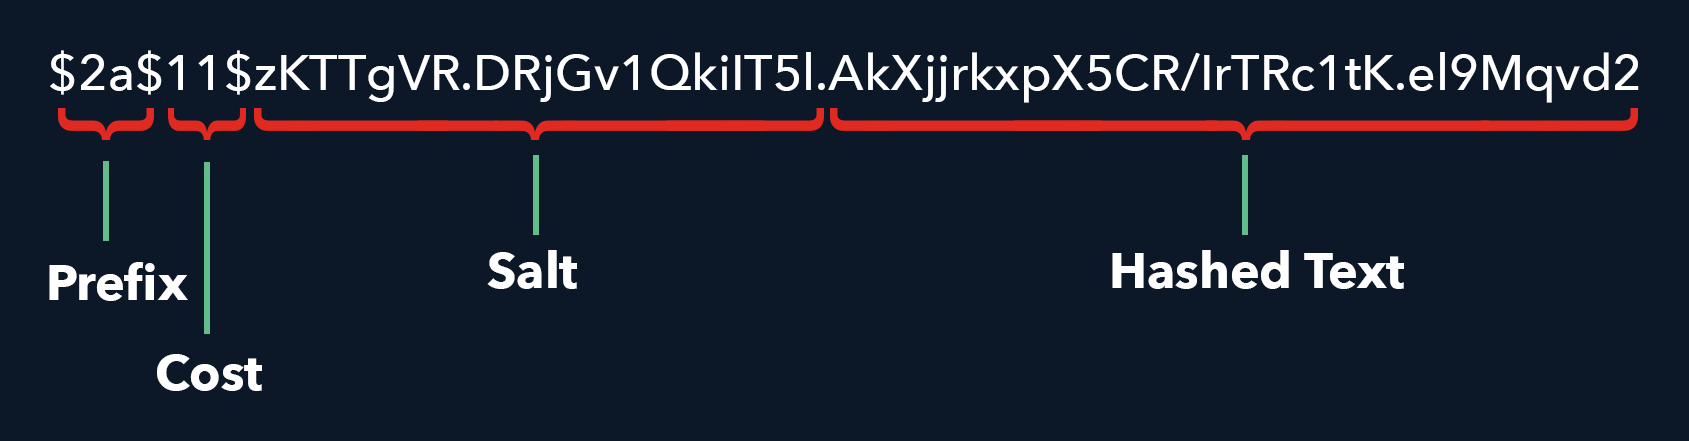
\includegraphics[width=\textwidth]{hash-anatomy}

\subsubsection{Cracking Hashes}
Depending on the operating system that you are on, you can find a tool to crack passwords.

\begin{description}
    \item[Windows] Cain and Abel: Strictly for Windows, it can crack numerous hash types including NTLM, NTLMv2, MD5, wireless, Oracle, MySQL, SQL Server, SHA1, SHA2, Cisco, VoIP, ando others
    \item[Linux] John the ripper
    \item[OSX] Various tools are available. John the ripper,
\end{description}

\end{document}

